\begin{frame}[fragile]
\frametitle{Episodes Covered}

\begin{itemize}
  \item \textbf{\# 226: The Price of Distraction} --- with Adam Gazzaley\\
        {\small Technology, attention, multitasking, and digital medicine}
  \item \textbf{\# 227: Knowing The Mind} --- with Steven Laureys\\
        {\small Meditation, free will, and the nature of the self}
  \item \textbf{\# 228: Doing Good} --- with William MacAskill\\
        {\small Effective altruism, charity, and the ethics of wealth}
\end{itemize}

\end{frame}

\section{\# 226: The Price of Distraction}

%%%%%%%%%%%%%%%%%%%%%%%%%%%%%%%%%%%%%%%%%%%%%%%%%%%%%%%%%%%%%%%%
\begin{frame}[fragile]
\frametitle{\# 226: The Price of Distraction}

\begin{center}
\textit{A Conversation with Adam Gazzaley}\\[4mm]
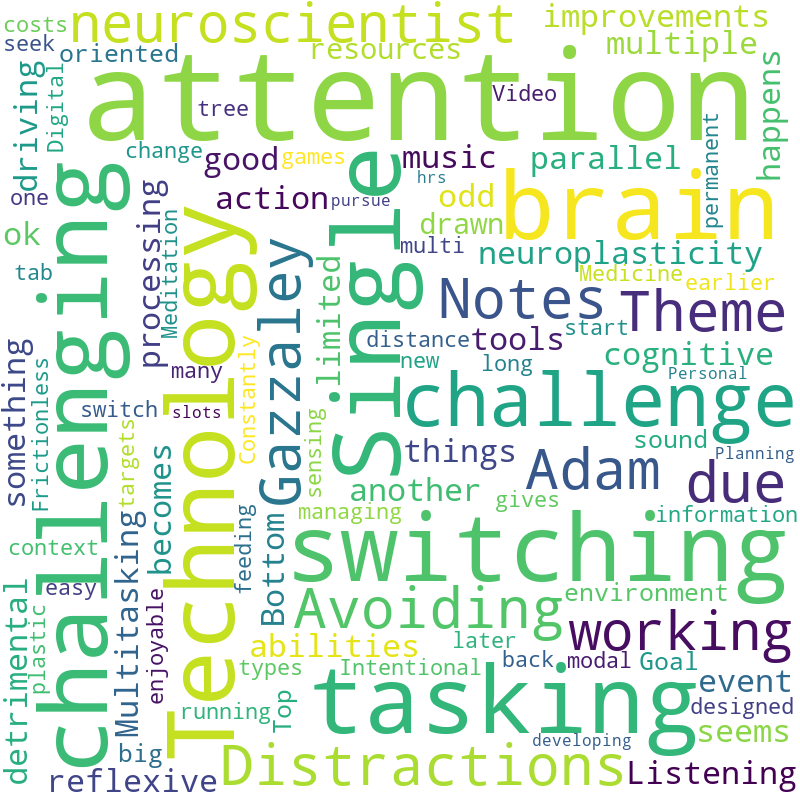
\includegraphics[width=0.55\linewidth,keepaspectratio]{images/Review_Podcast_MakingSense_226_PriceOfDistraction}
\end{center}

\end{frame}

%%%%%%%%%%%%%%%%%%%%%%%%%%%%%%%%%%%%%%%%%%%%%%%%%%%%%%%%%%%%%%%%
\begin{frame}[fragile]
\frametitle{\# 226: The Price of Distraction}

A Conversation with Adam Gazzaley

\begin{itemize}
\item Theme: Avoiding distractions caused by technology
\item Adam Gazzaley, neuroscientist working on neuroplasticity and tools for improving cognitive abilities
\item Multitasking: we enjoy doing multiple things, but the brain cannot truly parallel-process high-attention tasks.
\item Listening to music while doing a reflexive action like driving seems fine, but if something unexpected occurs, switching attention to it becomes dangerous.
\item Bottom-up attention: limited brain resources drawn by the environment, e.g.\ a sudden loud sound.
\item Top-down attention: goal-oriented and intentional.
\end{itemize}

\end{frame}

%%%%%%%%%%%%%%%%%%%%%%%%%%%%%%%%%%%%%%%%%%%%%%%%%%%%%%%%%%%%%%%%
\begin{frame}[fragile]
\frametitle{\# 226: The Price of Distraction}

\begin{itemize}
\item Constantly managing both attention types incurs switching costs to restore prior context.
\item Technology is designed to capture your attention. Each tab opens a new information tree; switching between them is frictionless.
\item Single-tasking: challenging to start but rewarding later, like long-distance running.
\item Digital Medicine: targeting specific brain challenges for neuroplastic change. Meditation is one example; video games use multimodal sensing to develop adaptive challenges.
\item Future of Technology: neural implants for extreme cognitive rehabilitation cases.
\end{itemize}

[Personal: Planning to pursue single-tasking in 2-hour slots]
\end{frame}

\section{\# 227: Knowing The Mind}

%%%%%%%%%%%%%%%%%%%%%%%%%%%%%%%%%%%%%%%%%%%%%%%%%%%%%%%%%%%%%%%%
\begin{frame}[fragile]
\frametitle{\# 227: Knowing The Mind}

\begin{center}
\textit{A Conversation with Steven Laureys}\\[4mm]
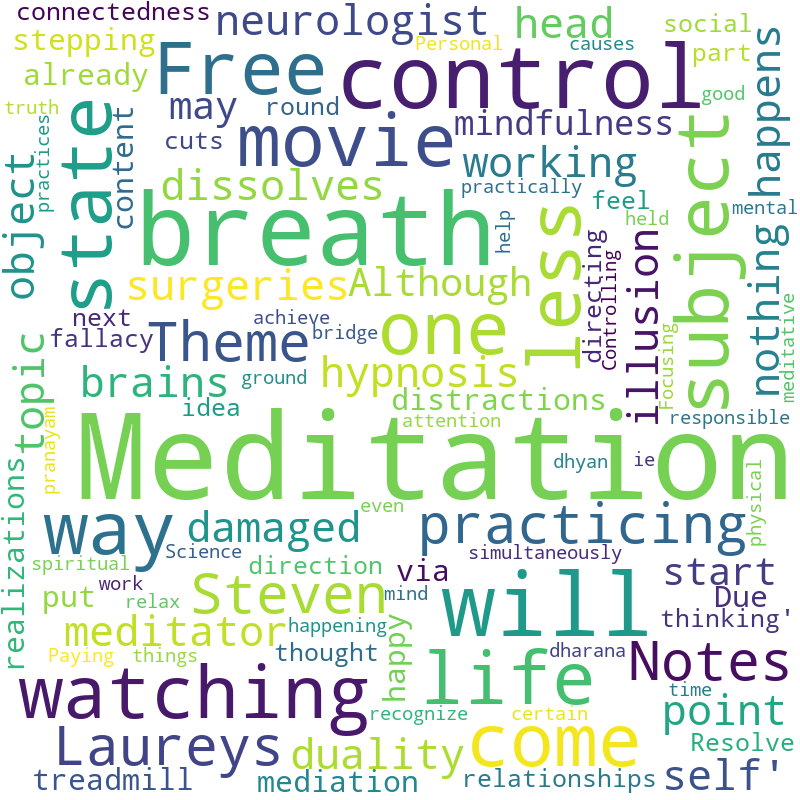
\includegraphics[width=0.55\linewidth,keepaspectratio]{images/Review_Podcast_MakingSense_227_KnowingTheMind}
\end{center}

\end{frame}

%%%%%%%%%%%%%%%%%%%%%%%%%%%%%%%%%%%%%%%%%%%%%%%%%%%%%%%%%%%%%%%%
\begin{frame}[fragile]
\frametitle{\# 227: Knowing The Mind}

A Conversation with Steven Laureys

\begin{itemize}
\item Theme: Meditation
\item Steven Laureys, practicing neurologist working on consciousness in damaged brains and surgeries under hypnosis.
\item Meditation: the subject-object duality is an illusion. At some point, the meditator and the object of meditation dissolve into one --- no control, it just happens.
\item There is nothing watching, no `self' in the head. You may start by watching the breath, but the meditative state arrives when mindfulness has no subject.
\item Meditation: doing less, stepping off the treadmill.
\item Through meditation you discover you are already content --- and bring that into relationships and social connectedness, not the other way round.
\end{itemize}

\end{frame}

%%%%%%%%%%%%%%%%%%%%%%%%%%%%%%%%%%%%%%%%%%%%%%%%%%%%%%%%%%%%%%%%
\begin{frame}[fragile]
\frametitle{\# 227: Knowing The Mind}

\begin{itemize}
\item Meditation dissolves the illusion that ``you'' are thinking. There is no Free Will in the classic sense.
\item Free Will: you have no control over which thought arises next. You feel you are directing the movie, but that direction is itself part of the movie.
\item Practical resolution: live a good life, do work, achieve things --- and simultaneously recognize it is all unfolding on its own (while still being held responsible for your actions in daily life).
\item Science is the ground truth even for spiritual practices: specific ways of paying attention are what produce the meditative state.
\end{itemize}

[Personal: Breath (pranayam) is the bridge from physical to mental. Controlling breath can relax the mind. Focusing on breath (dharana) helps enter a meditative state (dhyan).]
\end{frame}

\section{\# 228: Doing Good}

%%%%%%%%%%%%%%%%%%%%%%%%%%%%%%%%%%%%%%%%%%%%%%%%%%%%%%%%%%%%%%%%
\begin{frame}[fragile]
\frametitle{\# 228: Doing Good}

\begin{center}
\textit{A Conversation with William MacAskill}\\[4mm]
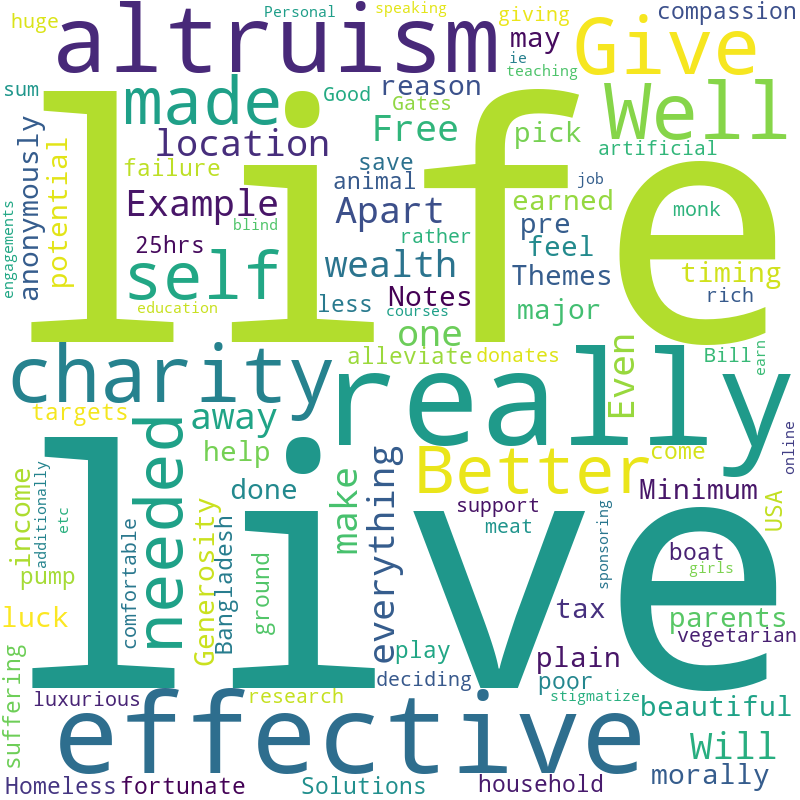
\includegraphics[width=0.55\linewidth,keepaspectratio]{images/Review_Podcast_MakingSense_228_DoingGood}
\end{center}

\end{frame}

%%%%%%%%%%%%%%%%%%%%%%%%%%%%%%%%%%%%%%%%%%%%%%%%%%%%%%%%%%%%%%%%
\begin{frame}[fragile]
\frametitle{\# 228: Doing Good}

A Conversation with William MacAskill

\begin{itemize}
\item Themes: Generosity, effective altruism.
\item Minimum 10\% of pre-tax income to the most effective charity (``Give-Well'' pledge).
\item Is giving better done anonymously? Not necessarily --- a public pledge can encourage others.
\item Altruism owed? You did not choose your location, parents, timing, or luck. In that sense you are not purely ``self''-made --- just as the ``will'' in Free Will may not be truly free.
\item Even if you feel you earned it, why not help? Have compassion for the less fortunate.
\end{itemize}

\end{frame}

%%%%%%%%%%%%%%%%%%%%%%%%%%%%%%%%%%%%%%%%%%%%%%%%%%%%%%%%%%%%%%%%
\begin{frame}[fragile]
\frametitle{\# 228: Doing Good}

\begin{itemize}
\item Charity solutions should come from the ground up. Example of failure: the PlayPump water carousel required children to play $\sim$27 hours/day to meet one household's water needs.
\item Who should charities target? The homeless in the USA or the extreme poor in Bangladesh? Effective altruism argues for the highest-impact use of each dollar.
\item Make the lifeboat more seaworthy so it can save more people.
\item To alleviate animal suffering: be vegetarian; support artificial meat research.
\item Good example: Bill Gates lives comfortably and donates enormous sums --- making generosity aspirational, not punishing. Don't stigmatize wealth.
\end{itemize}

[Personal: Apart from sponsoring a blind girl's education, I give away all earnings outside my job --- from speaking engagements, online courses, and teaching.]
\end{frame}
